\documentclass[a4paper,12pt, notitlepage]{article}

\usepackage[top=25mm,bottom=25mm,left=25mm,right=25mm]{geometry}
%\usepackage{amsmath} 
\usepackage{graphicx}
%\usepackage{epstopdf}
\usepackage{listings}
\usepackage{color}
\usepackage{url}
\usepackage{setspace} 
%\usepackage[square, numbers]{natbib}
\usepackage{titlesec}
\usepackage{fancyhdr}
\usepackage[export]{adjustbox}
\usepackage{wrapfig}
\usepackage[ddmmyyyy]{datetime}

\setstretch{1.44}
\setlength{\columnsep}{6mm}
\titleformat{\section}{\bfseries\large\scshape\filright}{\thesection}{1em}{}
\titleformat{\subsection}{\bfseries\normalsize\scshape\filright}{\thesubsection}{1em}{}

\renewcommand{\abstractname}{}
\newcommand{\captionfonts}{\footnotesize}
\renewcommand\thesection{\arabic{section}.}
\renewcommand\thesubsection{\arabic{section}.\arabic{subsection}}

\makeatletter
\long\def\@makecaption#1#2{
  \vskip\abovecaptionskip
  \sbox\@tempboxa{{\captionfonts #1: #2}}
  \ifdim \wd\@tempboxa >\hsize
    {\captionfonts #1: #2\par}
  \else
    \hbox to\hsize{\hfil\box\@tempboxa\hfil}
  \fi
  \vskip\belowcaptionskip}
    
\makeatother

\definecolor{dkgreen}{rgb}{0,0.6,0}
\definecolor{gray}{rgb}{0.5,0.5,0.5}
\definecolor{mauve}{rgb}{0.58,0,0.82}

\lstset{frame=tb,
	language=python,
	aboveskip=2mm,
	belowskip=2mm,
	showstringspaces=false,
	columns=flexible,
	basicstyle={\small\ttfamily},
	numbers=none,
	numberstyle=\tiny\color{gray},
	keywordstyle=\color{blue},
	commentstyle=\color{dkgreen},
	stringstyle=\color{mauve},
	breaklines=true,
	breakatwhitespace=true,
	tabsize=3
}

\pagestyle{fancy}
\fancyhf{}
\rhead{HILTOP Prod. Testing: Beginners Guide}
\lhead{\includegraphics[height=1cm]{./Images/logolong.png}}
\rfoot{Page \thepage}
\lfoot{}

\renewcommand{\dateseparator}{.}

\begin{document}
%%%%%%%%%%%%%%%%%%%%%%%%%%%%%%%%%%%%%%%%%%%%%%%%%%%%%%%%%%%%%%%%%%%%%%%%%%%%%%%%%%%%
\title{\textbf{\large{Beginners Guide to HILTOP Production Testing Framework}}}

\author{\normalsize{Devtank Ltd.} \\
        \small\textit{
        Harry Geyer}}
\date{\today}

\maketitle 
\thispagestyle{fancy}

%%%%%%%%%%%%%%%%%%%%%%%%%%%%%%%%%%%%%%%%%%%%%%%%%%%%%%%%%%%%%%%%%%%%%%%%%%%%%%%%%%%%
\begin{abstract} 
\noindent
A short guide for beginners to using the HILTOP Production Testing Framework. Covers device structure, test groups, global functions and database handling. 
\end{abstract}
%\vspace{11mm}

\tableofcontents
\newpage

%%%%%%%%%%%%%%%%%%%%%%%%%%%%%%%%%%%%%%%%%%%%%%%%%%%%%%%%%%%%%%%%%%%%%%%%%%%%%%%%%%%%
\section{Globals}
\label{sec: globals}

\subsection{Device}
\label{ssec: globalsDev}

The device under test is made into the python object, \url{dev}, and will contain the information to be tested in the scripts. It is constructed in \url{example_hw.py}, see Section \ref{sec: examplehw} The device is given a UUID which is a universally unique identifier that is assigned to a device but is expected to change, accounted for in database storage. The initial UUID is generated through random numbers but it is often replaced by hardware MAC address when found.

\subsection{Tests and Test Groups}
\label{globalTests}

Tests are arranged into test groups and these will be executed by the testing framework. Test groups are found in \url{./apps/app/tests/groups.yaml} and the group that will be used when the GUI is starts is set in \url{./apps/app/mb_prod_lib_gui/start_gui.py}. They are in simple yaml `default\_flow\_style' and the order of the tests will determine the order executed.

\subsection{Adjustable Arguments}
\label{ssec: globalsArgs}

Inside the \url{groups.yaml} file, arguments can be set for each test script. Argument `example' can be called by \lstinline{example = args["example"]}{. To create these arguments, they must be defined in \url{./apps/app/args.yaml} and given a type and description. Additional attributes can be given such as max, min, range and default where applicable. These arguments will be entered into the database for the associated device and test group. 

\subsection{Checks}
\label{ssec: globalsChecks}

Inside \url{./dtlib/pylibapps/dt_db_base/base_run_test_group.py} there are definitions of global functions that should be used in test scripts and in expanding the structure. There are three checks: \lstinline{test_check}{, \lstinline{exact_check}{ and \lstinline{threshold_check}{.

\begin{table}[h]
	\centering
	\begin{tabular}{ c c }
		\hline 
		Test & Arguments \\ %& Arg Type\\
		\hline 
		\url{test_check} & \url{(Bool, Name)} \\ %& \url{bool, str} \\ 
		\url{exact_check}  & \url{(Value, Ref Value, Name)} \\ %& \url{float, float, str} \\ 
		\url{threshold_check} & \url{(Value, Ref Value, Threshold, Unit, Name)} \\ %& \url{float, float, float, str, str} \\
		\hline 
	\end{tabular}
	\caption{Table of checks showing the arguments for each.}
	\label{tab: checks}
\end{table}

In Table \ref{tab: checks}, `Bool' is a boolean to test, `Name' is the name of the test to be recorded in the database, `Value' is a float to check, `RefValue' is the reference value (float), `Threshold' is the acceptible error and `Unit' is a string for unit of value. These checks will be written to the output file and if they fail, they will stop the script.

\subsection{Save to Database}
\label{ssec: globalsDatabase}

Information can be stored to the database with the function \lstinline{store_value("desc", value)}{ which will store \lstinline{value}{ with the name `desc' to the database associated with the device's serial number and test group. For more information how the database is constructed, see Section \ref{sec: Database}

\subsection{Outputs}
\label{ssec: globalsOutputs}

There are three set output commands to use: \lstinline{output_good}{, \lstinline{output_normal}{ and \lstinline{output_bad}{. These will print outputs in the `output' and `log' files to be displayed in \textit{Output} and \textit{Log} windows on the production tester GUI. All of these functions take a single argument as a string. These functions should be used for monitoring but will not stop a script.

There is a final output command, \lstinline{info_msg}{ that works similarally to \lstinline{output_normal}{ however writes to only the `log' file and so can only be seen in the \textit{Log} window.

%%%%%%%%%%%%%%%%%%%%%%%%%%%%%%%%%%%%%%%%%%%%%%%%%%%%%%%%%%%%%%%%%%%%%%%%%%%%%%%%%%%%

\newpage
\section{The Structure of dev}
\label{sec: examplehw}

\subsection{Overview}
\label{ssec: examplehwOverview}

\begin{wrapfigure}{r}{0.3\textwidth}
	\centering
	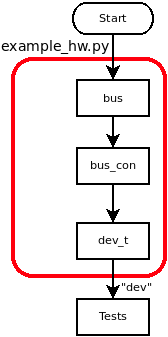
\includegraphics[width=50mm]{Images/examplehw.png}
	\caption{\small A flowchart showing the relationship between these three classes.}
	\label{fig: examplehw}
\end{wrapfigure}

The binding contains three of the core classes that are used to communicate with the hardware connected, although more can be added at your discretion. The example binding location is \url{./apps/app/example_lib/example_hw.py}.

The bus class contains attributes and functions for the bus. It is instantiated when the GUI opens and has “open” and “close” functions which are executed (pythonically) at the start and exit of the object (which is likely the start and end of the program).

This bus object is then handed to bus\_con to find the connection to the device by iterating over the devices on the bus connection. If there is a known UUID, it is handed to the dev\_t class as the dev object is made. The connection class is split with the bus class as there are some devices you may not want to power all the time.

The final class, dev\_t, contains attributes and functions of the device that will be used inside the test scripts. In the example this is just UUID and test functions (to be used in the class, not needed here for script). This class is the type of object that will be given to the test scripts, with object name `dev'. This object is also exposed to itself in the database. 

You may need to call functions in bus or bus\_con with arguments from scripts, this can be done by handing forward the self of bus or bus\_con, however when assigning use weakref to stop dependency loops.

Figure \ref{fig: examplehw} shows how the dev object is constructed from bus, bus\_con and then dev\_t. Contained inside the red line are the parts that are inside the example\_hw.py file. Arrows symbolise calling of classes, aside from Start to bus, these will be objects being constructed. 

\subsection{Examples}
\label{subsec: examplehwExamples}

Example of adding ssh with paramiko to dev object:
\begin{lstlisting}[caption={A simplified dev object to handle ssh connections},label={lst: examplehwExample0}]
import paramiko
class example_dev(object):
    def __init__(self, uuid):
        self._uuid             = uuid
        self.test_check        = None
        self.threshold_check = None
        self.exact_check       = None
        self.store_value       = None
        self.ssh               = None
        self.hostname          = "host"
        self.username          = "user"
        self.password          = "passwd"
    def ssh_setup(self):
        self.ssh = paramiko.SSHClient()
        self.ssh.set_missing_host_key_policy(paramiko.AutoAddPolicy())
        self.ssh.connect(hostname=self.hostname,
                           username=self.username,
                           password=self.password)
\end{lstlisting}

From the test scripts, once \lstinline{dev.ssh_setup}{ has been called, ssh commands can be sent with \lstinline{dev.ssh.execute_command("ls")}{. This object will be instantiated once per test run, so multiple ssh connections would not need to be made for multiple scripts. Any function used in multiple scripts should be placed here.

\begin{figure}[h]
	\begin{lstlisting}[caption={Simple script to setup ssh then use `ls' to remote.},label={lst: examplehwExample1a}]
dev.ssh_setup()
stdin,stdout,stderr = dev.ssh.execute_command("ls")
if not stdout.readlines():
     print("directory empty")
	\end{lstlisting}
	\begin{lstlisting}[caption={Using the existing ssh connection, this script checks usb ports.}, label={lst: examplehwExample1b}]
stdin,stdout,stderr = dev.ssh.execute_command("lsusb")
if not stdout.readlines():
     print("no usb ports")
	\end{lstlisting}
	\begin{lstlisting}[caption={This script changes some class attributes and opens a new ssh connection to a different remote.},label={lst: examplehwExample1c}]
dev.hostname = "diffhost"
dev.username = "user"
dev.password = "wouldntyouliketoknow"
dev.ssh_setup()
stdin,stdout,stderr = dev.ssh.execute_command("cat /proc/sys/kernel/hostname")
if stdout.readlines() != dev.hostname:
     print("hostname is ip not hostname")
     \end{lstlisting}
     \caption{Three test scripts showing how the structure constructed in Listing \ref{lst: examplehwExample0} can be used in the test scripts.}
     \label{lst: examplehwExample1}
\end{figure} 

With the scripts in Fig. \ref{lst: examplehwExample1} inside a test group, they would execute consecutively in the order defined in \url{groups.yaml}. In Listing \ref{lst: examplehwExample1c} it would be recommended to instead use \lstinline{dev.hostname = args["hostname"]}{ and so arguments could be given to the scripts, as described in Section \ref{ssec: globalsArgs}.
\newpage
\subsection{Building}
\label{ssec: buildingStruct}

While this document only touches on python parts of the production testing structure, there is also a significant amount comprised of C (for lower level mostly) and so a build is required. 

If being used on a non-specialised local machine this can be done by navigating to \url{./apps/app/} and first clearing the database (required when test scripts are added/groups ammended as these are stored in the database, see Section \ref{ssec: testsDatabase}) with \lstinline[language=bash]{make local_db_clean}. Once the database is cleaned, use \lstinline[language=bash]{make} to build and \lstinline{./output/bin/example_tester_gui.sh --production --desktop}{ to start the testing GUI. The arguments applied cause the GUI to run in production mode (not admin) and desktop (not full screen), respectively. 

If being run on a HILTOP then it should be built on startup, but you may need to update the test group list which is done by \lstinline{./output/bin/example_tester_gui.sh update_tests tests/calibration/your_test_group.yaml}{ with your\_test\_group.yaml being the group.yaml for your test group.

%%%%%%%%%%%%%%%%%%%%%%%%%%%%%%%%%%%%%%%%%%%%%%%%%%%%%%%%%%%%%%%%%%%%%%%%%%%%%%%%%%%%
\newpage
\section{Database}
\label{sec: Database}

The connected database can either be SQLite or MySQL, for local or remote functionality. On startup it will be set to MySQL, to change to SQLite use\newline \lstinline{./apps/app/output/bin/example_tester_gui.sh --config config_sqlite_db.yaml}{.

\subsection{Devices}
\label{ssec: devicesDatabase}

The key identifier for the devices in the database is the serial number used to scan the device. Once a device begins a test group, the results can be stored into the database and then reviewed later. If a device is rescanned then an option to review previous results will be displayed. There are four tables describing the device, but the most important table for per device review is `example\_dev\_test\_results' which contains device ID, test group ID, pass/fail, and the output and log file ID. If looking for individual values set in test scripts then `example\_dev\_test\_results\_values' is the table to query. 

\subsection{Test Groups}
\label{ssec: testsDatabase}

There are four tables for tests and test groups, one stores each test, one for storing the test group executed, one for storing the results of the test run and a final for the values collected in the test run. The latter two tables are the most important for finding results per test group. 

\subsection{Values}
\label{ssec: valuesDatabase}

Values inside the database are stored in the `values' table, it has an ID that is referenced in both results per test and results per device (tables `test\_group\_entry\_properties' and `example\_test\_results' respectively). 

%%%%%%%%%%%%%%%%%%%%%%%%%%%%%%%%%%%%%%%%%%%%%%%%%%%%%%%%%%%%%%%%%%%%%%%%%%%%%%%%%%%%
%\small{
%\begin{thebibliography}{99}

%\setlength{\itemsep}{-2mm}

%\bibitem{Webpage} Page Title,
%                  Author {\url{https://www.url.org/}} {Accessed: dd.mm.yy}.
%\bibitem{Book} Author, 
%                  {\em Book Name}. Publisher {\bf Edition}, Pages (Publish Year).
%
%\end{thebibliography}
%}
%
\end{document}